\chapter{Contribution \& system design}
\section{Work objectives}
\section{System Design}

In this section, we introduce our proposed voting system that aims to solve some of the barriers that traditional voting systems have.

\subsection{Architecture}

\begin{figure}[H]
	\centering
		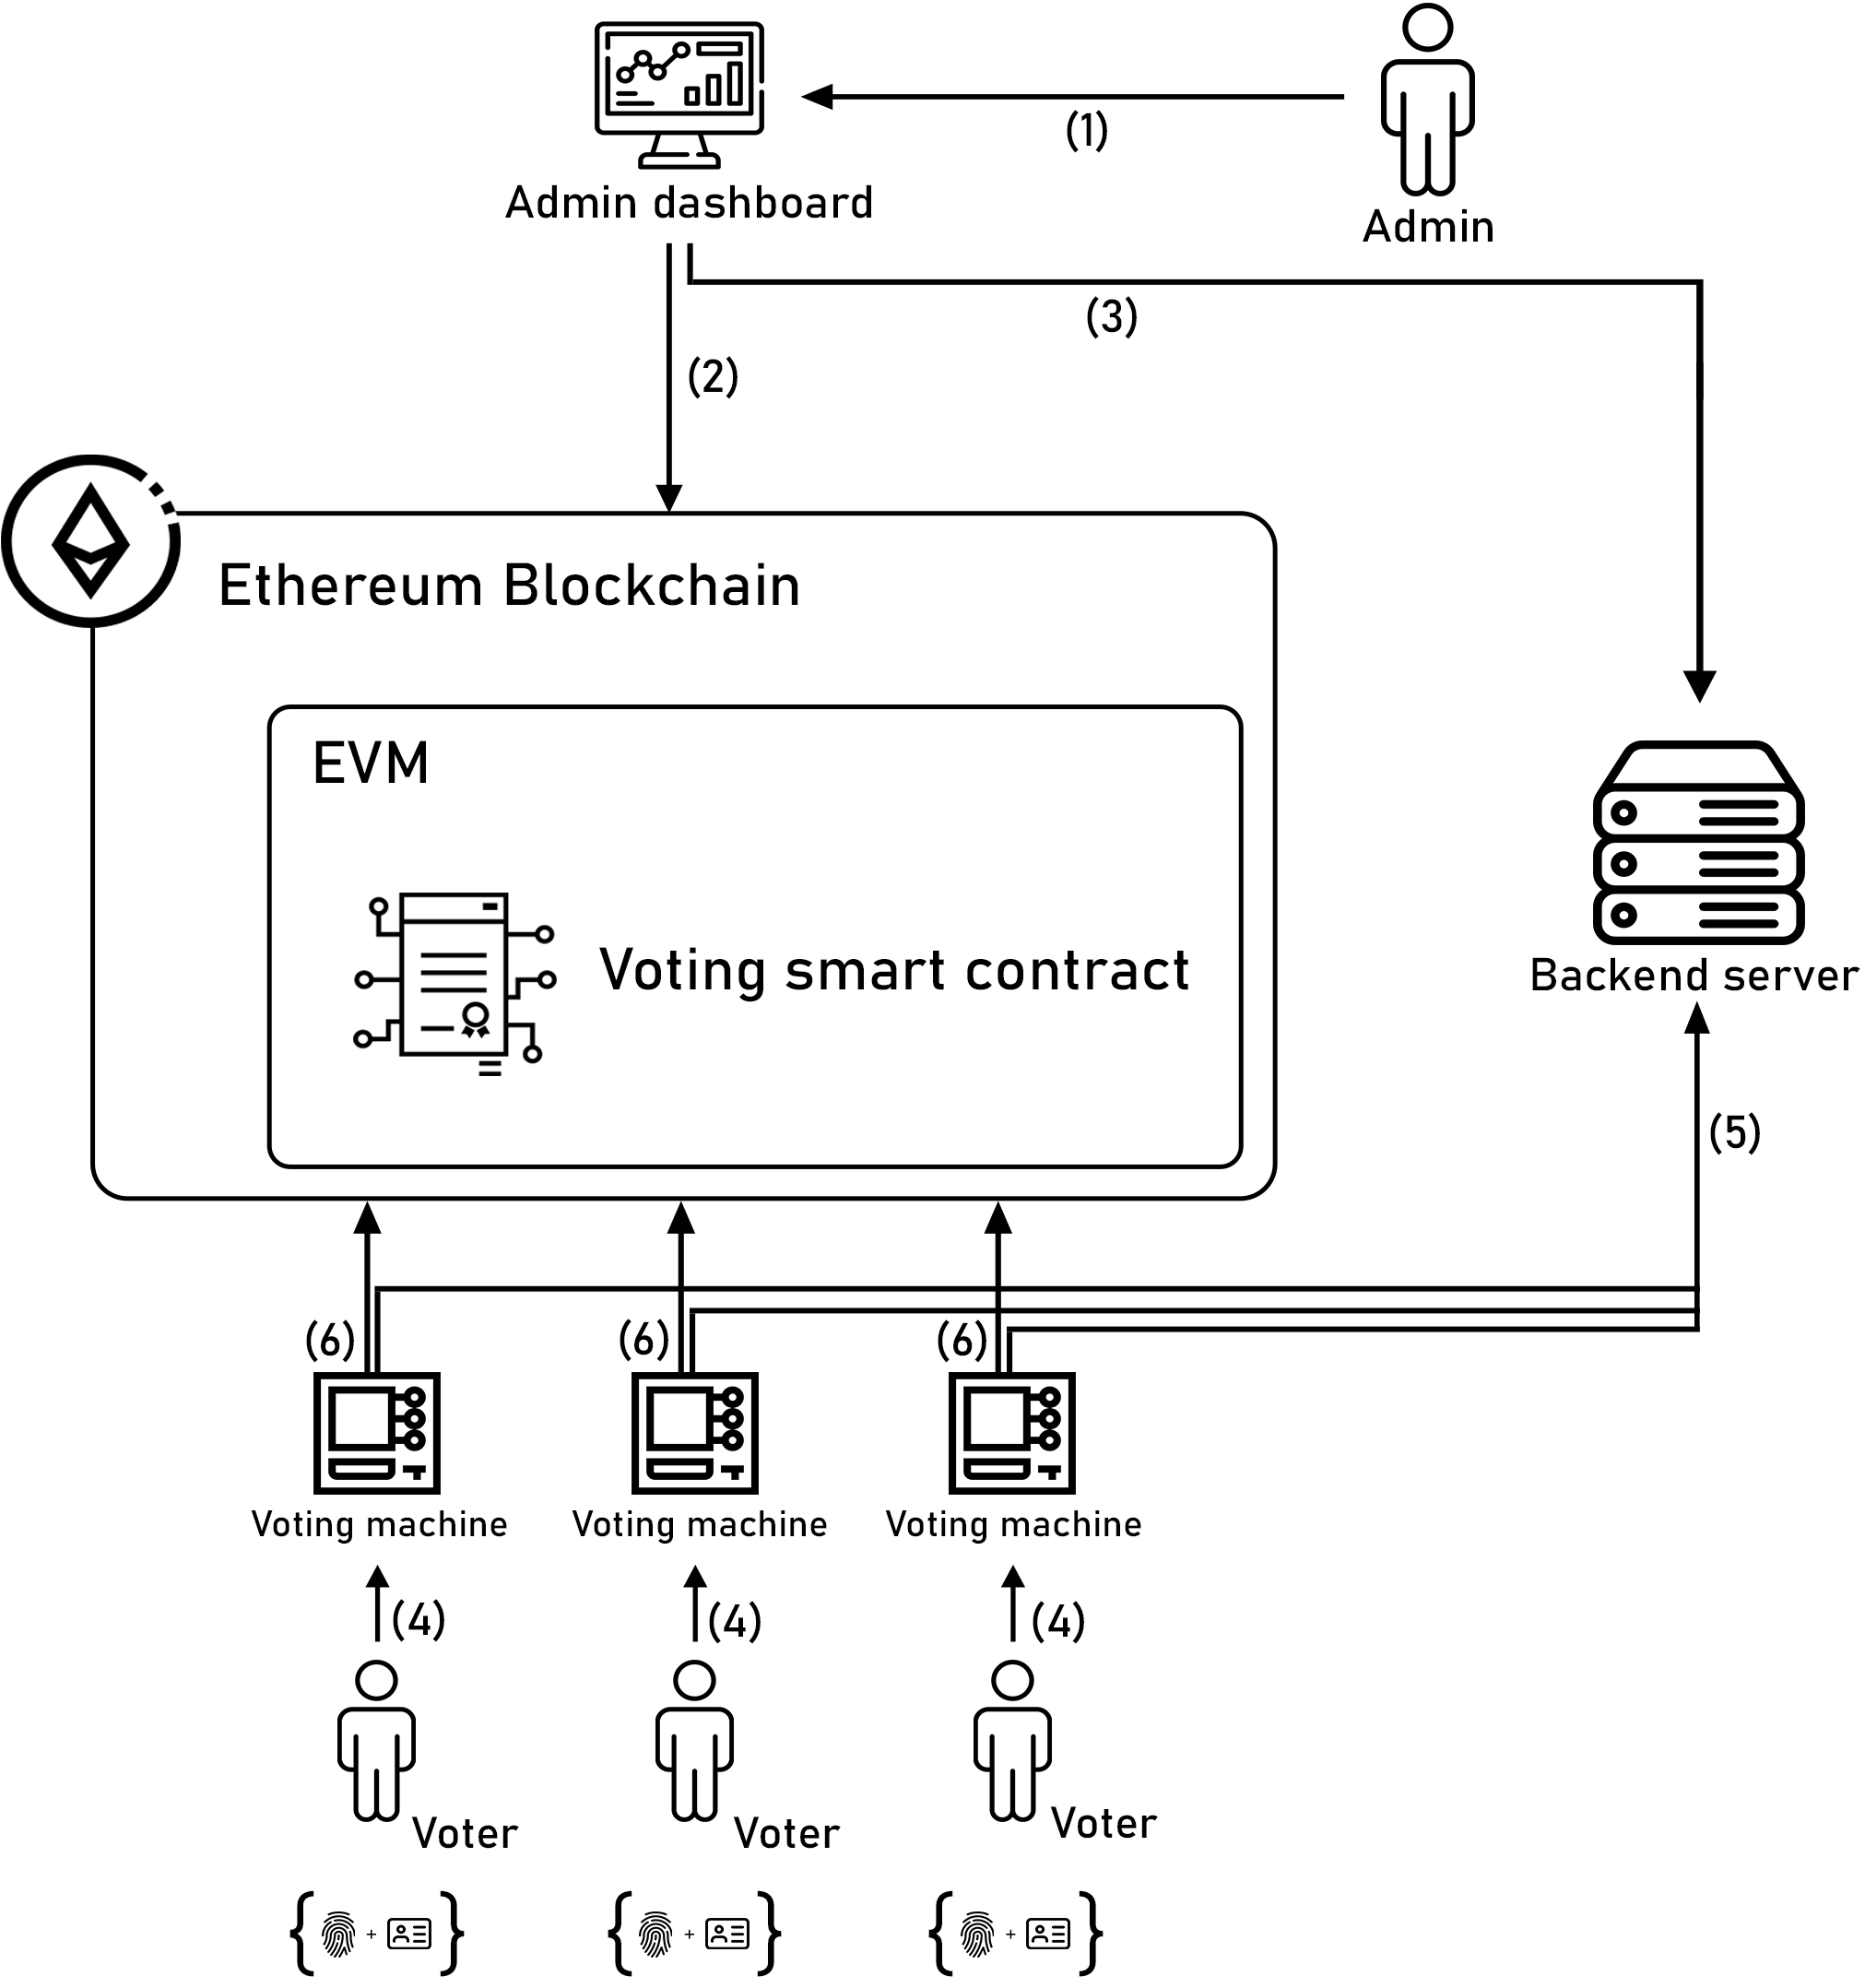
\includegraphics[width=12cm]{images/chapter3/architecture.png}
		\caption{{\footnotesize High level architecture of the proposed system and the interaction between its components}}
\end{figure}

\begin{list}{}{}
\item \textbf{(1)} The admin operating the dashboard launches and monitors voting events
\item \textbf{(2)} Essential data (candidates name and id, event title, start \& finish dates) are saved in the Blockchain along with the list of authorized accounts that can interact with the smart contract.
\item \textbf{(3)} Secondary data that is of less importance is saved to the regular (centralized) backend server.
\item \textbf{(4)} Voters authenticate themselves to the polling machines (using biometric means) and cast their vote for a candidate of their choosing
\item \textbf{(5)} Voting machines use the backend server to verify the identity of the voter and to fetch secondary data required for the displaying of candidates
\item \textbf{(6)} Voting machines saves the submitted choice to the Blockchain by launching a transaction that increments the vote count of the chosen candidate
\end{list}

\subsection{Diagrams}
\subsubsection{Admin sequence diagram}

\begin{figure}[H]
	\centering
		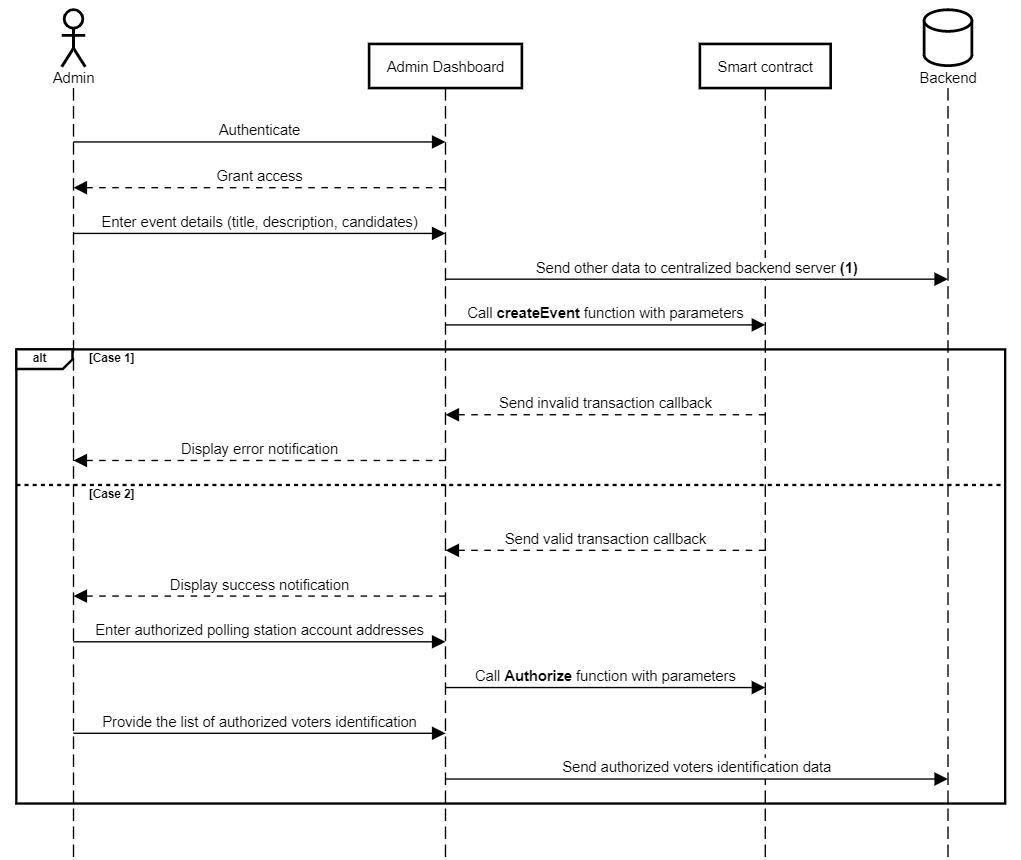
\includegraphics[width=14cm]{images/chapter3/admin_sequence_diagram.png}
		\caption{{\footnotesize Sequence diagram of the process of creating and launching a new voting event}}
\end{figure}

Launching an election requires that the administrator get access to the administration dashboard which has its access restricted by digital or physical boundaries or both, using the dashboard the administrator accesses the event creation form, in which he fills the information for the event. The information provided will be divided on the basis of their level of criticality, for example, candidates' pictures and lengthy descriptions are deemed to be less critical to the vote-counting so they're stored in a regular backend server. Also, information required for the authentication of voters is also stored on the regular backend servers.

Next, the administrator is tasked with providing the account addresses of the Ethereum accounts running on each voting machine, this list will be the list of the Ethereum account addresses allowed to interact with the smart contract and alter the vote count of any candidates by incrementing it.

\subsubsection{Voter sequence diagram}

\begin{figure}[H]
	\centering
		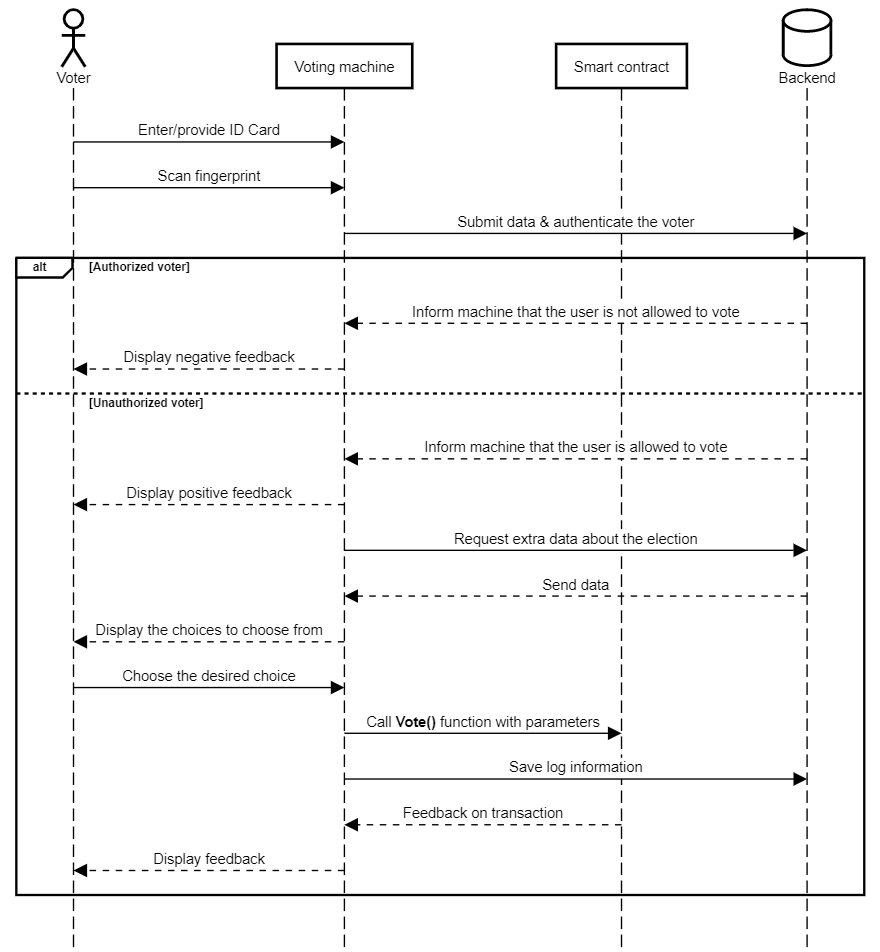
\includegraphics[width=14cm]{images/chapter3/voter_sequence_diagram.png}
		\caption{{\footnotesize Sequence diagram of the process of casting a vote}}
\end{figure}

The process of casting a vote is initiated when a voter first enters a polling station, then proceeds to a vacant voting machine, the machine should be equipped with an ID Card reader and fingerprint scanner to conduct a biometric identity check. the information obtained will be checked against the records saved on the backend server. In case the person is identified as an authorized voter; meeting whatever the requirements listed by the entity organizing the voting event (for example an entity can enforce one single vote per household or set the minimum age for participation to 50), a list of choices will be displayed to the voter to choose from in an intuitive manner after the voter makes his choice and submits it, the voting machine performance an Ethereum transaction to the smart contract by calling the appropriate function that will result in incrementing the vote count of that particular candidate, also log information about the vote will be saved to the backend server.
